% !TeX program = xelatex
% Copyright (c) 2026 handbookformyself contributors
% SPDX-License-Identifier: MIT
% 编译：latexmk -xelatex -outdir=output/pdf main.tex
\documentclass[a4paper,11pt,twoside]{article}
\usepackage{handbookformyself}










% 输出模式：电子版不留空白页；双面打印时改为 \printmodetrue。
\printmodefalse










% ECNU 配色示例：覆盖模板的功能色，不改变各命令的用途。
\definecolor{HBMain}{HTML}{A82338}
\definecolor{HBTime}{HTML}{3B637A}
\definecolor{HBTalk}{HTML}{745883}
\definecolor{HBBreak}{HTML}{4C7962}
\definecolor{HBNotice}{HTML}{B1722E}










% 页眉与 PDF 元数据。会议名、时间、地点直接写在使用位置。
\RunningTitle{ECNU / Example Workshop in Algebraic Geometry}
\hypersetup{pdftitle={Example Workshop in Algebraic Geometry},
  pdfauthor={handbookformyself},pdfsubject={Illustrative conference handbook}}










% 报告登记：题目、讲者与摘要各写一次；时间留给日程。
% 本示例的讲者和节目均为演示内容，不对应真实会议。
\DeclareTalk{curves}{
  speaker={Speaker A}, affiliation={Example Institute},
  title={Curves, line bundles and divisors}
}{
  A divisor on a smooth projective curve determines a line bundle, and sections
  of that bundle turn geometric questions into linear algebra. We begin with
  divisors on the projective line and then compare their behaviour on curves of
  positive genus. If $g$ is the genus of $C$, the Riemann--Roch formula reads:
  \[
    h^0(C,L)-h^0(C,K_C\otimes L^{-1})=\deg L+1-g.
  \]
  We use the formula to discuss effective divisors and maps to projective space.
  The examples require only the definitions of a divisor and a line bundle.
}

% affiliation 可以省略；这一项同时演示题目中的数学。
\DeclareTalk{positivity}{
  speaker={Speaker B},
  title={Positivity and projective embeddings of $X$}
}{
  An ample line bundle records how a projective variety can be embedded into
  projective space after taking a suitable tensor power. We compare ampleness
  and global generation using line bundles on curves and on projective space.
  In particular, the bundles $\mathcal O_{\mathbb P^n}(d)$ give a concrete family
  in which sections and the associated morphisms can be described explicitly.

  The second part follows the same questions through simple constructions:
  restricting a line bundle to a subvariety, taking tensor products, and pulling
  back sections along a morphism. These examples separate the geometric role of
  an embedding from the algebraic description of its coordinate sections.
}

% 长题目、多段正文、公式与列表都可以直接放入摘要。
\DeclareTalk{families}{
  speaker={Speaker C}, affiliation={Example University},
  title={Families of projective varieties and the geometric meaning of specialization in moduli problems}
}{
  A family organizes several algebraic varieties into a single geometric
  object. Our running example is the family of plane conics
  \[
    \mathcal X=\{x_0x_1=t x_2^2\}
      \subset \mathbb P^2\times\mathbb A^1,
    \qquad \pi:\mathcal X\longrightarrow\mathbb A^1.
  \]
  For nonzero $t$ the fiber is a smooth conic, while the fiber over zero is the
  union of two lines. This small example makes specialization visible without
  requiring a general construction of a moduli space.

  \Needspace{4\baselineskip}
  We will keep track of two questions throughout the discussion:
  \begin{enumerate}
    \item Which features can be read from a single fiber?
    \item Which questions require the total space and the map $\pi$?
  \end{enumerate}
  We finish by comparing different choices of the parameter and explaining why
  a description of the fibers alone does not describe the whole family.
}

\DeclareTalk{bundles}{
  speaker={Speaker D}, affiliation={Example Research Centre},
  title={Vector bundles on projective space and a first look at splitting}
}{
  On the projective line, every vector bundle is a direct sum of line bundles:
  \[
    E\cong\bigoplus_{i=1}^{r}\mathcal O_{\mathbb P^1}(a_i).
  \]
  We discuss how the integers $a_i$ describe sections and restrictions, and why
  the higher-dimensional problem has a different character. The Euler sequence
  \[
    0\longrightarrow\mathcal O_{\mathbb P^n}
      \longrightarrow\mathcal O_{\mathbb P^n}(1)^{\oplus(n+1)}
      \longrightarrow T_{\mathbb P^n}\longrightarrow0
  \]
  supplies a familiar bundle with which to test the same questions.
}

\DeclareTalk{dynamics}{
  speaker={Speaker E}, affiliation={Example Institute},
  title={Pullback, degree growth and elementary examples in algebraic dynamics}
}{
  Iterating an algebraic map gives a sequence of pullbacks. For an
  endomorphism $f:\mathbb P^k\to\mathbb P^k$ of algebraic degree $d$, the
  hyperplane class $H$ satisfies $f^*H=dH$ and the iterates have degree $d^n$.
  We use this calculation to connect iteration with linear algebra on
  cohomology.

  The talk compares these projective-space examples with maps on curves.
  The aim is to identify which quantities are being measured before moving to
  more general varieties and rational self-maps. Notation for sheaves, such as
  $\mathcal E$ and $\mathscr F$, will be introduced when it is needed.
}










\begin{document}
% 封面不编号，且不与正文第 1 页共用自动页面锚点。
\hypersetup{pageanchor=false}
\pagenumbering{gobble}

% 完整封面保留在内容文件中，换会议时可直接替换此块。
\begin{titlepage}
  \thispagestyle{empty}
  \setlength{\parskip}{0pt}
  \raggedright
  \pdfbookmark[0]{Example Workshop in Algebraic Geometry}{example.cover}
  \begin{minipage}[c]{0.5\linewidth}
    \small\color{HBMuted}School of Mathematical Sciences
  \end{minipage}\hfill
  \begin{minipage}[c]{0.45\linewidth}\raggedleft
    
\includegraphics[width=\linewidth]{assets/ecnu-logo.png}
  \end{minipage}\par
  \vspace{18mm}
  {\color{HBMain}\rule{24mm}{4pt}\par}
  \vspace{5mm}
  {\bfseries\fontsize{31}{35}\selectfont\color{HBMain}
    Example Workshop in\\Algebraic Geometry\par}
  \vspace{4mm}
  {\Large\color{HBMuted}A handbookformyself demonstration\par}
  \vspace{12mm}
  {\bfseries\HandbookIcon{day}\quad Friday / 20 November 2026\par}
  \vspace{3mm}
  {\HandbookIcon{clock}\quad09:00--15:10 / Shanghai time\par}
  \vspace{6mm}
  {\bfseries\HandbookIcon{location}\quad East China Normal University\par}
  \vspace{2mm}
  {\small\color{HBMuted}Mathematics Building / Example programme\par}
  \vspace{6mm}
  {\small\HandbookIcon{info}\quad Illustrative event, speakers and room labels\par}
  \vfill
  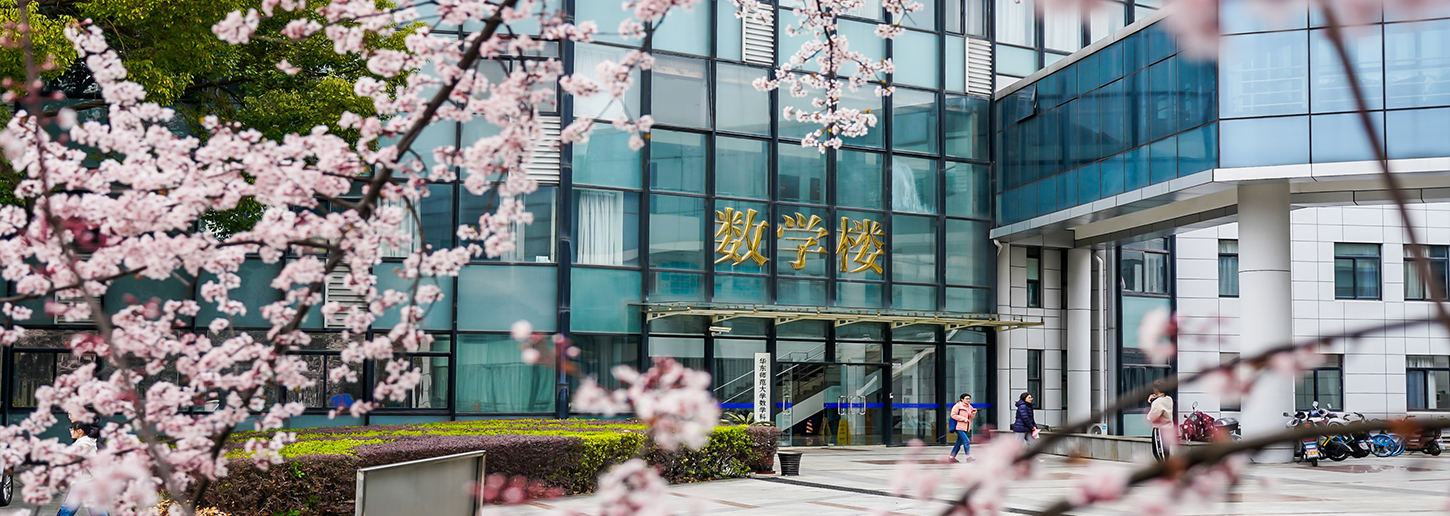
\includegraphics[width=\linewidth]{assets/ecnu-math-building.jpg}\par
  \vspace{2mm}
  {\fontsize{8}{10}\selectfont\color{HBMuted}
    Photograph: School of Mathematical Sciences, ECNU\par}
\end{titlepage}

% 打印版的封面背面留白；两种模式的正文都从第 1 页编号。
\ifprintmode
  \null\thispagestyle{empty}\newpage
\fi
\pagenumbering{arabic}
\hypersetup{pageanchor=true}










% 目录也是普通正文；各大分段自动登记目录项。
\tableofcontents
\markright{Contents}
\clearpage










% 会议须知：五种白底 box 都能独立使用，也允许内容自然跨页。
\HandbookSection{Meeting information}[An illustrative programme for a small mathematics workshop]

\begin{infobox}[Venue and registration]
  The programme uses the Mathematics Building at ECNU as its visual setting.
  Speaker names, times and room labels are examples for adapting the template.
  Registration opens at 08:40 in the example foyer.

  \textbf{中文示例：}本手册中的讲者、日程及房间名称均为演示内容。
\end{infobox}

\begin{sessionbox}[Session format]
  Each talk has a forty-minute slot, including questions. Morning and afternoon
  are separate sessions; the programme below gives the order explicitly.
\end{sessionbox}

\begin{talkbox}[Notes for speakers]
  Please include the title and speaker name on the first slide. A short board
  discussion is welcome after the presentation.
\end{talkbox}

\begin{noticebox}[Before the session]
  Check the display connection before your talk. Any change to a title belongs
  in the final programme, so please send corrections to the organisers before
  the session begins.
\end{noticebox}

\begin{breakbox}[Refreshments]
  Coffee is served in the example foyer. The midday break gives participants
  time to eat nearby, and the final discussion brings both sessions together.
\end{breakbox}

\HandbookSubsection[\faIcon{users}]{Contact and organisers}
For this demonstration, use \href{mailto:organiser@example.org}{organiser@example.org}
as the placeholder contact address. Replace it with the organisers' address
when preparing a real handbook.










% 日程：时间不放进 DeclareTalk，而是在使用报告 ID 时填写。
\clearpage
\HandbookSection[HBTime]{Schedule}[Friday / 20 November 2026]

\HandbookSubsection[\faIcon{users}]{Morning}[09:00--11:30 / Example lecture room]
\ScheduleItem{09:00--09:40}{curves}
\ScheduleBreak[coffee]{09:40--10:00}{Coffee and informal discussion}
\ScheduleItem{10:00--10:40}{positivity}
\ScheduleBreak{10:40--10:50}{Interval}
\ScheduleItem{10:50--11:30}{families}
\ScheduleBreak[meal]{11:30--13:00}{Midday break}

\HandbookSubsection{Afternoon}[13:00--15:10 / Example lecture room]
\ScheduleItem{13:00--13:40}{bundles}
\ScheduleBreak{13:40--14:00}{Interval}
\ScheduleItem{14:00--14:40}{dynamics}
\ScheduleBreak[discussion]{14:40--15:10}{Open discussion: questions from the talks and ideas for future collaboration}










% 摘要：原来的报告数据直接复用；示例允许公式、列表与多段正文。
\clearpage
\HandbookSection[HBTalk]{Abstracts}
\HandbookSubsection{Morning}
\TalkAbstract{curves}
\TalkAbstract{positivity}
\TalkAbstract{families}

\HandbookSubsection{Afternoon}
\TalkAbstract{bundles}
\TalkAbstract{dynamics}










% 后勤页：使用普通 LaTeX、表格和原生 TikZ，不需要额外的数据文件。
\clearpage
\HandbookSection[HBBreak]{Logistics}[Example arrangements and an illustrative floor plan]

\HandbookSubsection[\faIcon{map}]{Venue plan}
The following drawing illustrates how a venue plan can be included directly in
the content file. Its room labels and route are demonstration data.

\begin{center}
\begin{tikzpicture}[x=1cm,y=1cm,font=\small]
  \draw[HBMain,line width=0.7pt] (0,0) rectangle (14,4.6);
  \draw[HBMain!50] (0,1.4)--(14,1.4);
  \draw[HBMain!50] (4.5,1.4)--(4.5,4.6) (9.5,1.4)--(9.5,4.6);
  \node[align=center,text=HBBreak] at (2.25,3) {Coffee area\\\HandbookIcon{coffee}};
  \node[align=center,text=HBTalk] at (7,3) {Example lecture room\\\HandbookIcon{talk}};
  \node[align=center,text=HBMain] at (11.75,3) {Discussion room\\\HandbookIcon{discussion}};
  \node at (2,0.7) {Entrance};
  \draw[->,HBTime,line width=0.8pt] (3.2,0.7)--(7,0.7)--(7,1.2);
  \node[text=HBMuted] at (11.3,0.7) {Illustrative corridor};
\end{tikzpicture}
\end{center}

\HandbookSubsection[\HandbookIcon{meal}]{Meals and accommodation}
\begin{infobox}[Arrangements to replace]
  \begin{description}
    \item[Meals] Insert confirmed dining locations and service times.
    \item[Accommodation] Add the hotel name, address and check-in information.
    \item[Transport] Add the appropriate station, campus gate and walking route.
  \end{description}
\end{infobox}

\HandbookSubsection[\faIcon[regular]{clock}]{Travel checklist}[Allow time to reach the meeting room]
\begin{enumerate}
  \item Check the venue address and the campus entrance before departure.
  \item Save a local copy of the programme and contact information.
  \item Tell the organisers about accessibility or equipment requirements.
\end{enumerate}










% 没有预设类型的新栏目：标题与内容仍由 main.tex 决定。
\clearpage
\HandbookSection[HBMuted]{Further notes}[A free-form section]

\HandbookSubsection{Discussion questions}
Use ordinary paragraphs, lists and equations for material that needs no special
box. A new section does not require a new style command or a new data registry.

\begin{itemize}
  \item Which examples connect two of the talks?
  \item Which hypotheses are needed for the displayed formulas?
  \item Which questions should be recorded for a follow-up meeting?
\end{itemize}

\HandbookSubsection[\HandbookIcon{info}]{About this example}
This booklet demonstrates the public commands of \texttt{handbookformyself}.
The contents and the schematic plan are original demonstration material.
The ECNU logo and building photograph are credited separately in
\texttt{assets/SOURCES.md}.

\begin{noticebox}[Adapting the handbook]
  Change the cover directly, choose the output mode near the beginning of this
  file, and replace the report declarations. Then list their IDs in the desired
  order in the programme and the abstract section.
\end{noticebox}

\end{document}
